In this chapter, we will look at the design of the state estimation and the vehicle platform it will be deployed to. The state estimation is built from the ground up, so there is a lot of flexibility regarding the design choices. The design is deliberately described in terms of generic components, enabling adoption on other platforms and software environments.

\section{Vehicle Platform}
The state estimation described in this thesis will be deployed to two electric \gls{4wd} race cars:
\begin{itemize}
\item a non-autonomous race car which is newly designed and manufactured
\item an autonomous race car which is already existing but repurposed
\end{itemize}
These vehicles will in the following be referred to as \gls{ev} and \gls{dv}, respectively. Note that the \gls{dv} is electric as well but has additional components required for autonomous driving.

\subsection{Sensor Setup}
The vehicles are equipped with a plethora of sensors, which can be used for state estimation. While some sensors like the ones for brake pressure are not relevant, most provide useful information. The relevant sensors are listed in table \ref{tab:sensor}, with the last two columns denoting in which vehicle they are available. The sensors' locations in the vehicle shown in figure \ref{fig:sensor-locations} In the ideal case, both vehicles would have the all sensors, since working with a homogeneous set of measurements is simpler, but financial and weight considerations mean that only the sensors necessary for the vehicle's use case are available.

\begin{table}[h]
	\newcommand\heading[1]{\textcolor{white}{\textbf{#1}}}
	\renewcommand{\arraystretch}{1.2}
	\sffamily
	\centering
	\begin{tabularx}{\textwidth}{X l c c}
	\rowcolor{black} \heading{Sensor type} & \heading{Measured variables~~~} & \heading{~EV~} & \heading{~DV~} \vspace{2pt} \\
	\Glsdesc{imu} with gyrometer & $a, \omega$ & \xmark & \xmark \\
	Optical cross-correlation velocity sensor & $v, \beta$ & \xmark &  \\
	\Glsdesc{gnss} & $p, \norm{v}$ & \xmark & \xmark \\
	\Glsdesc{gnss} & $\psi$ &  & \xmark \\
	Motor speed sensor & $\omega_{motor}$ & \xmark & \xmark
	\end{tabularx}
	\caption{Sensor setups for \gls{ev} and \gls{dv}}
	\label{tab:sensor}
\end{table}

\begin{figure}[h]
	\centering
	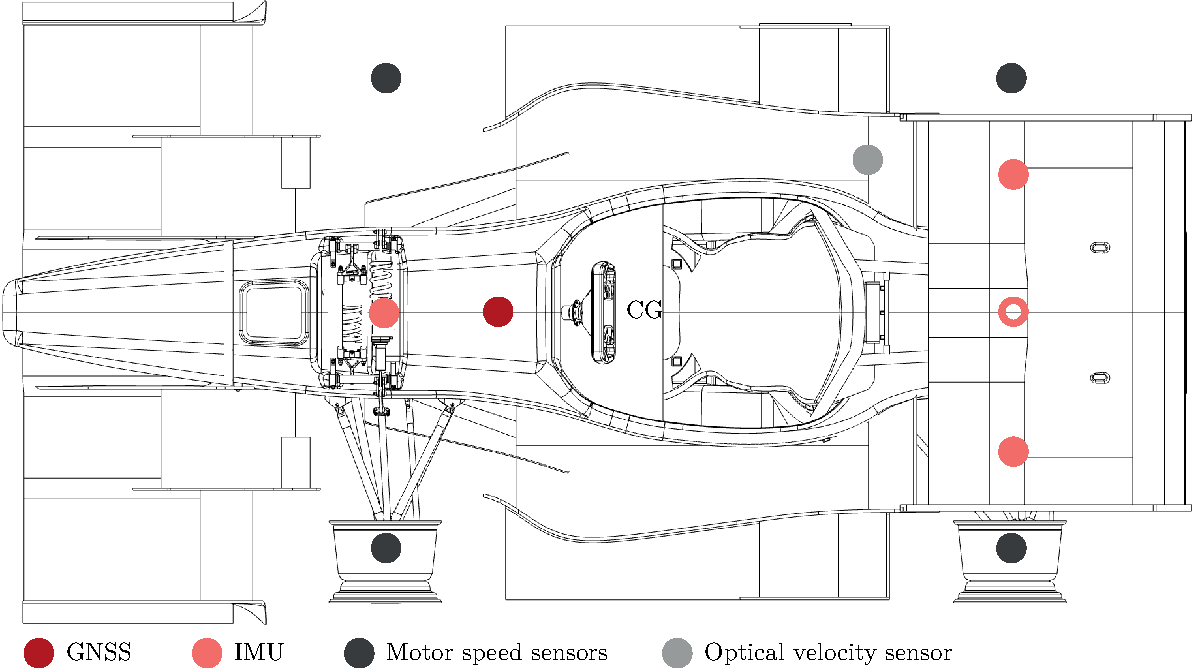
\includegraphics[width=\textwidth]{sensor_locations}%
	\caption{Locations of sensors in vehicle}
	\label{fig:sensor-locations}
\end{figure}

\begin{description}
\item[IMU] The \gls{ev} features three \glspl{imu} with gyrometers: one directly in front of the \gls{cog}, and two situated on the rear left and right. This enables redundancy, since accelerations and rotations in the two-dimensional plane only require two \glspl{imu}. In the \gls{dv}, the front one remains while only a single rear one, denoted by the circle with the missing center, is located directly behind the \gls{cog}. While these sensors react very fast, the signals are rather noisy~\cite[p.~19~ff.]{Biel.2019}.

\item[Optical velocity sensor] The optical cross-correlation velocity sensor, only available in the \gls{ev}, provides longitudinal and lateral speed measurements, and therefore also measurements of the vehicle sideslip angle. It enables slip-free velocity measurements by correlating photosensor information of the surface over time, which uniquely determines the speed and direction of movement~\cite{Bellof.4241993}. The fact that it is not influenced by slip, as velocity measurements from wheel speeds are, makes it a very valuable addition to the sensor setup. However, it is noisy and prone to temporary spikes and even failures on feature-less surfaces (see dark red line in figure \ref{fig:velocities} at \SI{5.2}{\second}).

\item[GNSS] A \gls{gnss} receiver is mounted in the front of both vehicles. Next to position measurements, they provide another source of speed information. The position accuracy is high in the range of a few centimeters. However, they are slow to react, with over \SI{100}{\milli\second} of delay in some situations~\cite[p.~27]{Biel.2019} (see dark grey line in figure \ref{fig:velocities}). The receiver mounted in the \gls{dv} additionally provides heading information, made possible by the relative position of two separated antennas mounted in the front and rear. This enables transformation of the speed into a velocity vector.

\item[Motor speed sensor] The rotary encoders in each of the four motors give individual rotation speed measurements for the four wheels. They are available in both vehicles and are assumed to be reliable, since the vehicle will not drive when they fail. However, when using them to calculate the vehicle velocity, deviations due to slip occur in highly dynamic situations (see light grey line in figure \ref{fig:velocities} at \SI{3.8}{\second})
\end{description}

\begin{figure}
	\centering
	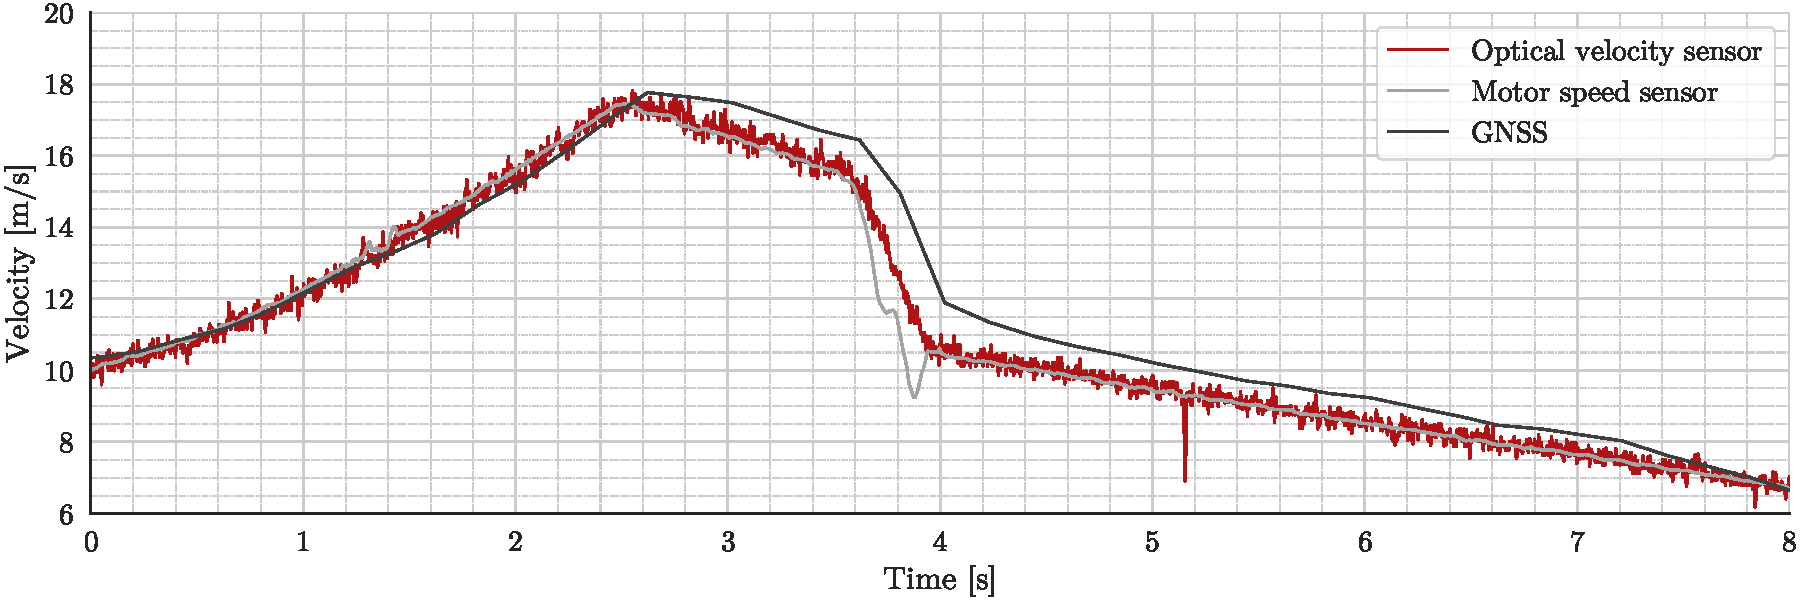
\includegraphics[width=\textwidth]{plot_velocities}%
	\caption{Comparison of velocity measurements from different sensors}
	\label{fig:velocities}
\end{figure}

To summarize, the key differences between the \gls{ev} and \gls{dv} are as follows:
\begin{itemize}
\item Three \glspl{imu} in \gls{ev} but two \glspl{imu} in \gls{dv}
\item No optical cross-correlation velocity sensor in \gls{dv}
\item No heading information in \gls{ev}
\end{itemize}
The lack of the optical velocity sensor in the \gls{dv} is inconvenient but not fatal, since the state estimation can compensate it. For track and obstacle recognition, the autonomous \gls{dv} is furthermore equipped with stereo cameras and lidar sensors. These could be used for optical flow computations to gain more position, attitude and velocity information, but for this design, we rely solely on the sensors described in the previous paragraphs. The estimated state is, however, used to correct lidar measurements.


\subsection{Computation System}\ref{sec:design-computation-system}
All sensor and control signals converge at the central \gls{ecu}. The software running on that \gls{ecu} is called \gls{vdc} and has several important tasks:
\begin{itemize}
\item Receive driver input from steering wheel and pedals
\item Send torque requests to each of the four motors
\item Limit speed and torque depending on situation
\item Increase vehicle agility through \gls{tv}
\item Optimize use of tire potential through \gls{tc}
\end{itemize}
Ultimately, the \gls{vdc}'s task is to help the driver to exploit the maximum physical potential of the vehicle through its \gls{tv} and \gls{tc}, collectively called \gls{perfcomp}.

\begin{figure}
	\centering
	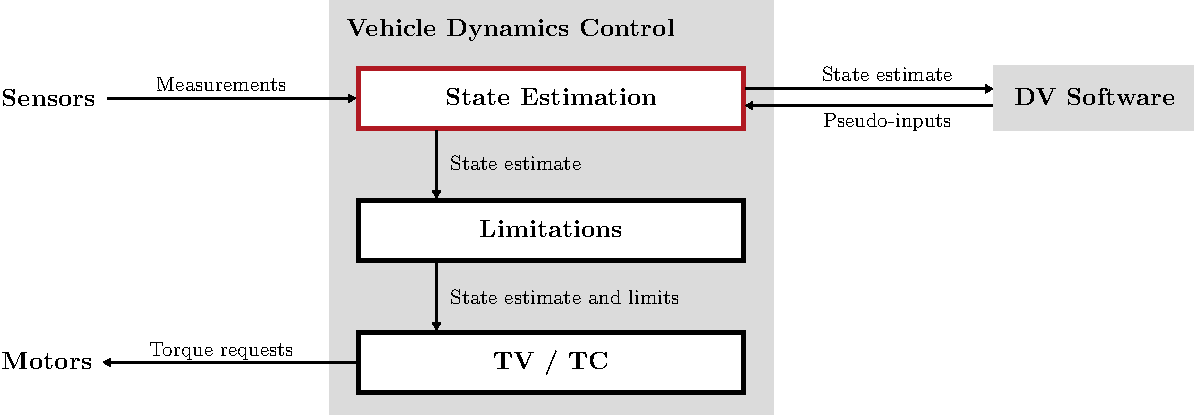
\includegraphics[width=\textwidth]{architecture_integration}%
	\caption{Integration of state estimation in software/hardware system}
	\label{fig:architecture-integration}
\end{figure}

The state estimation is located between the sensor inputs and the aforementioned \gls{perfcomp}, and is therefore part of the \gls{vdc} as well. The integration with input and output signals is shown in figure \ref{fig:architecture-integration}. While the \gls{vdc} is executed at a fixed rate, sensor inputs may arrive via a \gls{can} bus system at different rates. For example, the \gls{vdc} runs at \SI{1000}{\hertz}, i.e. it is scheduled to be executed every \SI{1}{\milli\second}, but optical velocity sensor measurements may arrive at \SI{250}{\hertz} and \gls{gnss} measurements even slower at \SI{5}{\hertz}. This may be due to a measurement overhead, such as satellite communication in case of the \gls{gnss}, which prohibits higher rates, but it may also be a conscious choice to reduce bus load and thus congestion. The state estimation must be able to fuse these measurements at different rates while providing continuous estimates at the highest rate. The time since the arrival of the last measurement is provided to aid this task.

Note that the software to control autonomous driving in the \gls{dv} runs on a separate, more powerful computer, which receives the state estimate from the \gls{ecu}. The \gls{ecu} then receives pseudo-driver inputs back from the motion controller and sends torque requests to the motors. However, the interface with the \gls{dv} software is beyond the scope of this thesis.


\section{Requirements}
goal: provide robust, accurate estimate of vehicle state for \gls{vdc} and DV software 
flexible: support arbitrary sensor setups within full sensor setup
robust: detect and handle sensor failures
state variables to estimate
estimate these variables in CoG, this describes motion of vehicle since it is assumed to be a rigid body
real-time: needs to be computable in 1 ms frequency
complete in all areas, so no developments in near future are necessary

design principle: use simple methods if they work just as well (occam's razor)
only if the results are not adequate, try more complicated approaches
easier to understand and troubleshoot
make less assumptions and thus generalize better
because maintainers change every year
on a higher level, clear architecture to facilitate maintenance and extension

We assume that vertical dynamics are negligible and only motion in the two-dimensional plane of the track are relevant, simplifying equations.

\section{Architecture}
in the literature, there is no concrete solution for our problem
however, we can combine common components into our own solution

At high level: state estimation = preprocessing + outlier detection + state estimation
To fulfill requirements of robustness and accuracy: outlier detection and sensor fusion
For practical reasons: preprocessing
preprocessing and outlier detection for each sensor in parallel
all IMUs have same treatment
out bus creation calculates vehicle side slip angle from vx and vy

For flexibility: outlier detection and sensor setup detection using same mechanism
in both cases, sensor cannot or should not be used in sensor fusion
does not matter if not connected, not sending, invalid values

\begin{figure}[h]
	\centering
	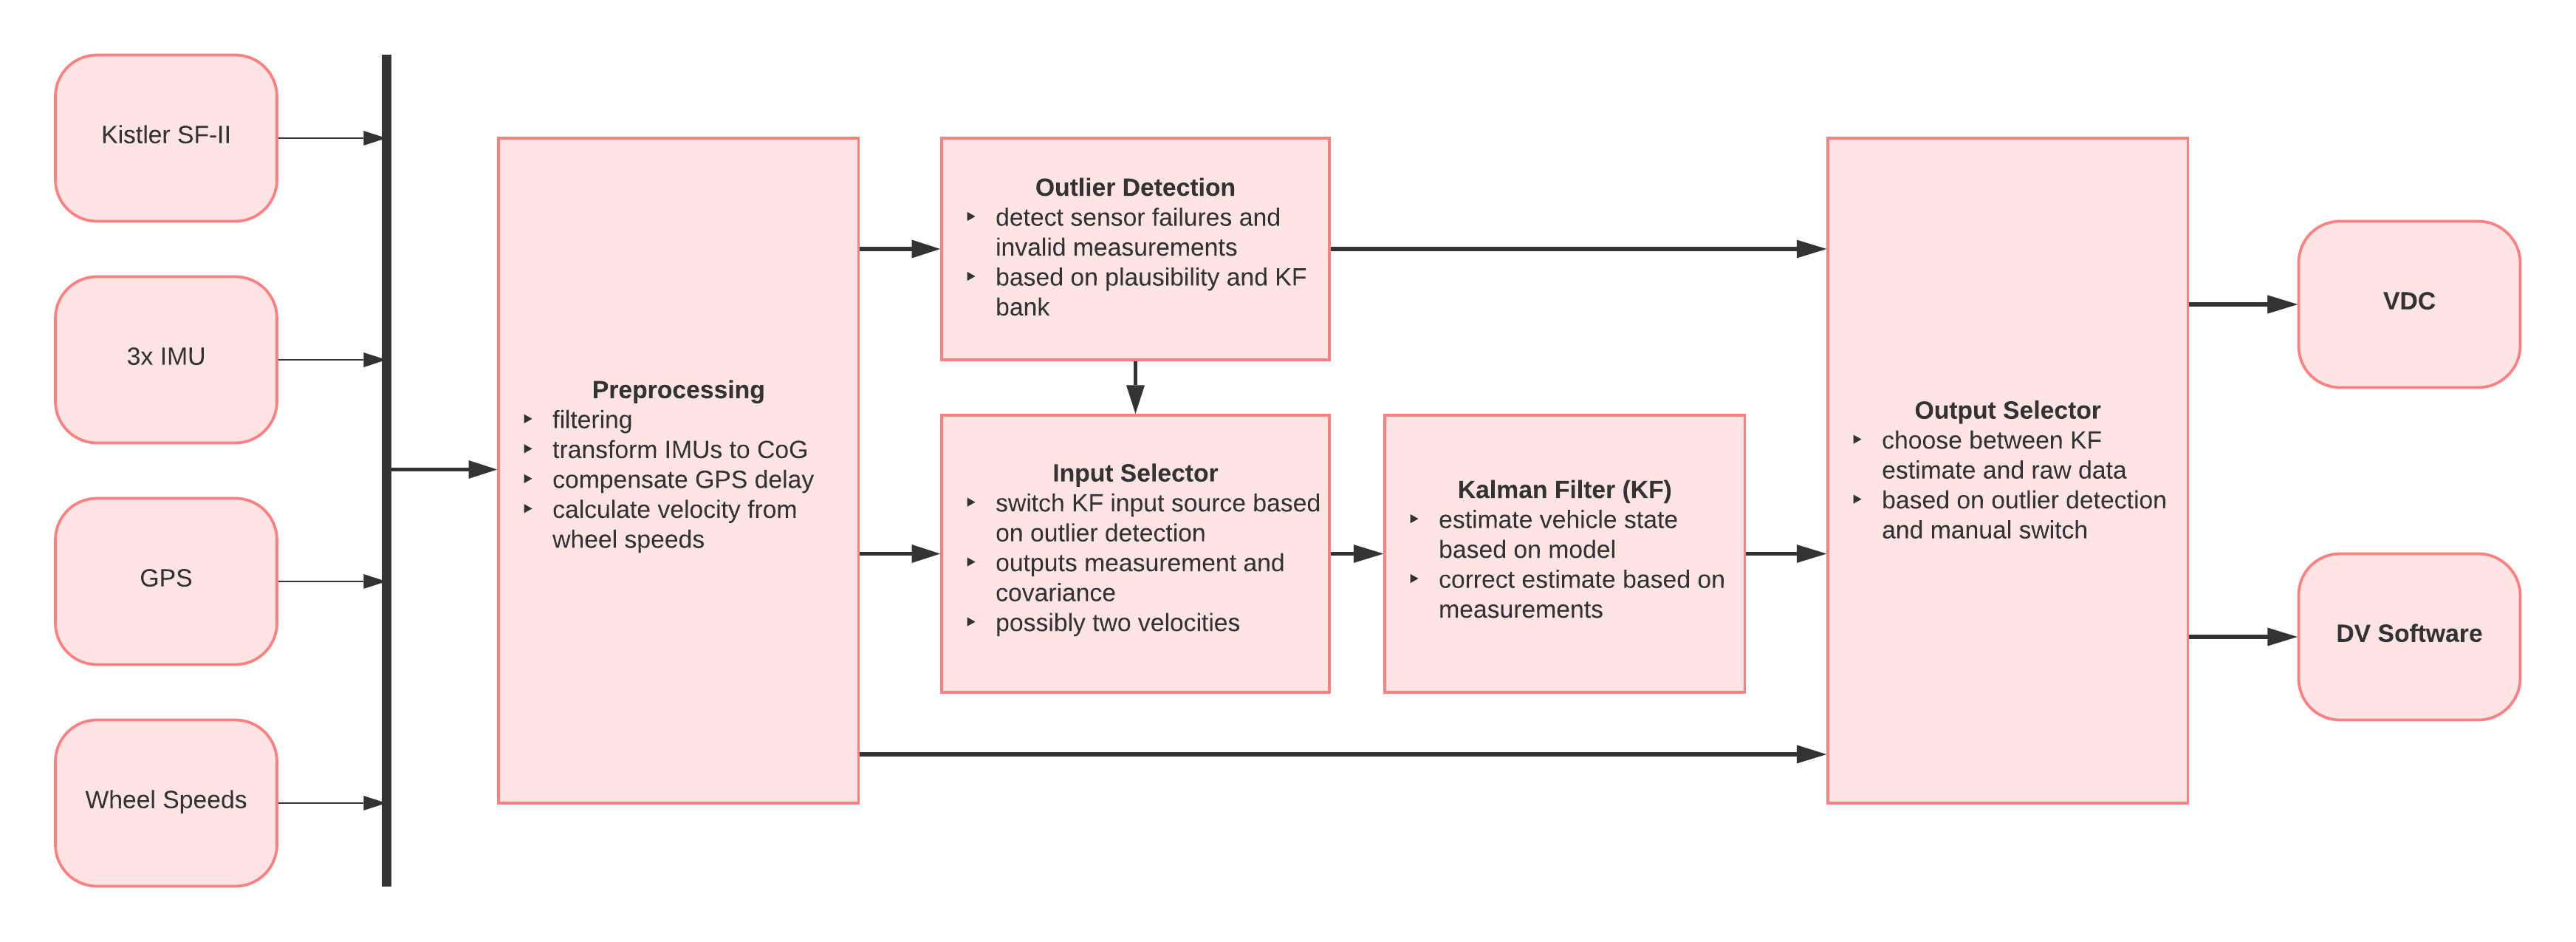
\includegraphics[width=\textwidth]{architecture}%
	\caption{High-level architecture}
	\label{fig:architecture}
\end{figure}
Show all inputs and outputs

\section{Preprocessing}
convert to SI units and deg to rad so formulas can be applied
show necessary transformations for each measurement

IMU fusion
very important because used extensively in EKF and other parts of VDC like TC and TV (especially dpsi)
fast response
contains outlier detection because available sensors need to be known before fusion in preprocessing
handle arbitrary number and position

GPS WGS84 coordinates transformed to track with first known point as origin

sfii transformed to \gls{cog}

\section{Outlier Detection}
Show diagram of AND and OR
For all EKF inputs
Plausibility check for all
For velocity, use wheels, GPS and sfii in EKF bank, different covs than in normal EKF
Plausibility for velocities rather conservative
observability and controllability
goal: support one sensor failure, more is unlikely

debouncing to increase robustness
allow manual three-way override to enable/disable sensors and override outlier detection errors

\section{EKF}
outlier detection sensor state is used to create measurement mask
Show input selection and state equations, jacobians
euler forward discretization
GPS is not included because it is not beneficial due to its slow response
kinematic model from~\cite[p.~156]{AlexanderWischnewski.2019}
reduces effects of noise
no heading measurements in ev, especially lack of initial heading is bad

prediction using differential equation
initialization
disable measurements using separate mask
input cov as process noise
